% Page settings
\documentclass[a4paper, 12pt]{article}                                     % Define the document page
\usepackage{setspace}                                                      % Space between lines (customisable)
\usepackage[margin=2.54cm]{geometry}                                       % Set margins (standard is 2.54cm)
\usepackage[UKenglish]{babel}                                              % Set default language
\usepackage[UKenglish,cleanlook]{isodate}                                  % Set default date and date display
\usepackage[activate={true,nocompatibility},final,tracking=true,kerning=true,spacing=true,factor=1100,stretch=10,shrink=10]{microtype}
\microtypecontext{spacing=nonfrench}                                       % Change font and minor spacings to look nicer
\setlength{\parskip}{0.5\baselineskip}                                     % Set default paragraph behaviour: skip a line
%% Packages to use:
% Tables + figures
\usepackage{graphicx}                                                      % control over the import of graphics
\usepackage[table,dvipsnames]{xcolor}                                      % Define tables (with colour control)
\usepackage{multirow}
\usepackage{float}                                                         % Control over graphics + tables float
\usepackage[justify]{ragged2e}                                             % control over text alignment
\usepackage{booktabs}                                                      % caption graphics + tables (with name in bold)
\usepackage[labelfont=bf]{caption}                                         % caption graphics + tables (with name in bold)
\usepackage{dcolumn} \newcolumntype{d}[1]{D..{#1}}                         % Common type of decimal column in tables.
\usepackage{tikz} \usetikzlibrary{automata,positioning}                    % Draw graphs inline, guide: https://sites.google.com/site/kochiuyu/Tikz
\definecolor{ao(english)}{rgb}{0.0, 0.5, 0.0}                              % Define dark green colour 
\usepackage{subcaption}                                                    % Sub figures.
% Maths + numbers
\usepackage{mathtools}                                                     % Various maths functions
\usepackage{amssymb}                                                       % Various maths functions
\usepackage{amsmath}                                                       % Various maths functions
\usepackage{dsfont}                                                        % Various maths functions
\usepackage{centernot}                                                     % center \not usage
\usepackage{siunitx} \sisetup{round-mode=places, round-precision=3}        % Formalise use of units and numbers among text
\usepackage{amsthm}                                                        % \DeclareMathOperator{\all}{,\; \text{ for }}                                    % all (with spacing) in equation shortcut
\renewcommand{\vec}[1]{\boldsymbol{\mathit{#1}}}                           % vector notation shortcut
\newcommand{\mat}[1]{\boldsymbol{\mathit{#1}}}                             % matrix notation shortcut
\DeclarePairedDelimiter\abs{\lvert}{\rvert}                                % absolute value notation shortcut
\DeclarePairedDelimiter\norm{\lVert}{\rVert}                               % norm notation shortcut
\newcommand{\Prob}[1]{\Pr\left( #1 \right)}                         % SHortcut for probability notation
\newcommand{\Probgiven}[2]{\Pr\left( #1 \, \middle\vert \, #2 \right)} % SHortcut for probability notation, given
\newcommand{\E}[2][]{\mathbb{E}_{#1} \left[ #2 \right]}                    % Expectation (with optional subscript) shortcut
\newcommand{\Egiven}[3][]{\mathbb{E}_{#1} \left[ #2 \, \middle\vert \, #3 \right]} % Expectation given (with optional subscript) shortcut
\newcommand{\Var}[2][]{\text{Var}_{#1} \left( #2 \right)}                  % Variation (with optional subscript) shortcut
\newcommand{\Cov}[1]{\text{Cov} \left( #1 \right)}                         % Covariance (with optional subscript) shortcut
\newcommand{\median}[1]{\text{median} \left( #1 \right)}                   % Median (with optional subscript) shortcut
\newcommand{\indicator}[1]{\mathds{1}\left\{ #1 \right\}}                  % SHortcut for indicator function
\newcommand{\diff}[2][]{\frac{d#1}{d#2}}                                   % SHortcut for differential fraction as a function
\newcommand{\partialdiff}[2][]{\frac{\partial#1}{\partial#2}}              % SHortcut for partial differential fraction as a function
\newcommand{\converge}[1]{\xrightarrow{ #1 \to\infty}}                     % SHortcut for convergence arrow
\renewcommand{\hat}[1]{\widehat{#1}}                                       % Default estimator notation is widehat
\renewcommand{\bar}[1]{\overline{#1}}                                      % Make over bar look nicer
\renewcommand{\tilde}[1]{\widetilde{#1}}                                   % Make over tilde look better
\newcommand{\indep}{\raisebox{0.05em}{\rotatebox[origin=c]{90}{$\models$}}}% Statistical independence symbol.
% Citations
\usepackage[longnamesfirst]{natbib}                                        % Citation package, see https://en.wikibooks.org/wiki/LaTeX/Bibliography_Management#Natbib
\usepackage[backref=page]{hyperref}                                        % Allow for links across the text, with colour options
\hypersetup{colorlinks=true, linkcolor=blue, citecolor=blue, filecolor=magenta, urlcolor=blue}
\def\sectionautorefname~#1\null{Section~#1\null}                           % Fix autoref for sections
\def\subsectionautorefname~#1\null{Subsection~#1\null}                     % Fix autoref for subsections
\def\subsubsectionautorefname~#1\null{Subsubsection~#1\null}               % Fix autoref for subsubsections
\def\equationautorefname~#1\null{Equation~(#1)\null}                       % Fix autoref for equations
% IMPORTANT: follow style guide here https://github.com/Wookai/paper-tips-and-tricks
\begin{document}
\noindent
\textbf{Simulation: Causal Mediation with Selection}
\hfill
\cleanlookdateon \today \\
Senan Hogan-Hennessy, \href{mailto:seh325@cornell.edu}{\nolinkurl{seh325@cornell.edu}}
\hfill
Cornell University
\rule{\textwidth}{0.4pt}

\noindent
This document investigates a system where a randomised measure $Z$ affects an outcome $Y$ via two channels: directly $Z \to Y$, and indirectly via a mediator $D(Z) \to Y$.

Causal mediation methods decompose the effect of $Z$ into indirect effects, the proportion of effect going through the $D(Z) \to Y$ channel, and direct effects, the $Z \to Y$ channel.
Conventional methods assume that $D$ is randomly assigned, conditional on $Z$ and other observed covariates $\vec X_i$; this assumption is unlikely to hold in observation settings, such as relying on quasi-experimental variation in $Z$.

This document simulates a system where $D$ is not randomly assigned, but is the result of Roy-style selection (based on treatment gains) involving observed selection factors $\vec X_i$ and unobserved $U_i$.
It shows how conventional estimators, controlling only for observed $\vec X_i$ behave under different assumptions about the distribution of $U_i$.

\section{Notation}
Write $Y_i$ for the observed outcome value e.g., long-run income, for individuals $i = 1, \dots, N$.
Suppose $Y_i$ is the outcome of two binary variables, $Z_i = 0,1$ which is assigned randomly, and $D_i = 0,1$ which individuals \textbf{select into} based on which $Z$ value they receive.
The researcher observes $D_i, Y_i$, but not their respective potential outcomes:
\begin{align*}
    D_i &= Z_i       D_i(1)
        + (1 - Z_i) D_i(0), \\
        &= \begin{cases}
            D_i(1), \text{ if } Z_i = 1 \\
            D_i(0), \text{ if } Z_i = 0
        \end{cases}  \\
    Y_i &= Z_i      Y_i(1, D_i(1))
        + (1 - Z_i) Y_i(0, D_i(0)) \\
        &= \begin{cases}
            Y_i(1, 1), \text{ if } Z_i = 1, D_i(1) = 1 \\
            Y_i(1, 0), \text{ if } Z_i = 1, D_i(1) = 0 \\
            Y_i(0, 1), \text{ if } Z_i = 0, D_i(0) = 1 \\
            Y_i(0, 0), \text{ if } Z_i = 0, D_i(0) = 0
        \end{cases}.
\end{align*}
In my empirical work, $Z$ is a binary version of the gene score for education (differenced from parents' values, EA score), $D_i(Z_i)$ is a choice to complete higher education, and $Y_i$ a measure of long-run income.
$\vec X_i$ is demographic information, gender, age, and every measure of socio-economic standing available; $U_i$ is covariates the \textbf{researcher wants to control for, but does not observe} in the data they have.

\begin{figure}[h!]
    \centering
    \singlespacing
    \caption{Structural Causal Graph of the Triangular System, $Z\to D\to Y$.}
    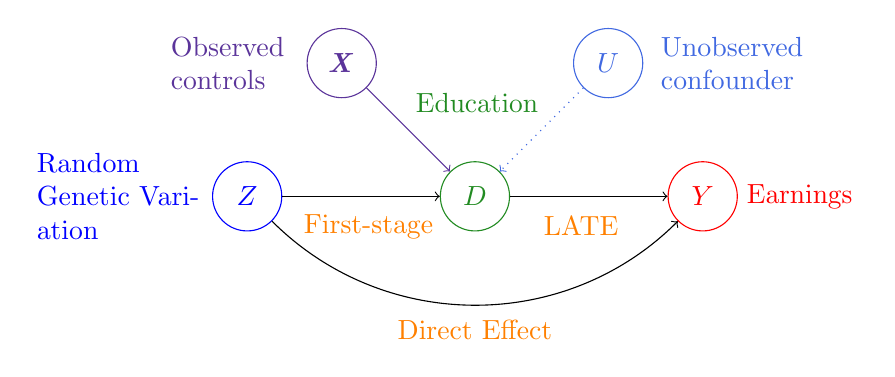
\begin{tikzpicture}
        \node[state,ForestGreen] (treatment) at (0,0) {$D$};
        \node[state,blue] (instrument) [left=2cm of treatment] {$Z$};
        \node[state,red] (outcome) [right=2cm of treatment] {$Y$};
        \path[->] (instrument) edge (treatment);
        \path[->] (treatment) edge (outcome);
        % Label the nodes with econ examples
        \node[text width=2cm, color=blue] [left=0.1cm of instrument] {Random Genetic Variation};
        \node[text width=0.1cm, color=red] [right=-0.01cm of outcome] {Earnings};
        \node[text width=1.5cm, color=ForestGreen] [above=0.5cm of treatment] {Education};
        % Add in direct effects.
        \path[->] (instrument) edge[bend right=45] (outcome);
        % Label the causal effects
        \node[text height=1cm, color=orange] [left=0.5cm of outcome] {LATE};
        \node[text height=1cm, color=orange] [right=0.15cm of instrument] {First-stage};
        \node[text height=1cm, color=orange] [below=0.25cm of treatment] {Direct Effect};
        % Add in the confounders
        \node[state,RoyalPurple] (confounderX) [above left=1.5cm of treatment] {$\vec{X}$};
        \path[->,RoyalPurple] (confounderX) edge (treatment);
        \node[text width=1.5cm, color=RoyalPurple] [left=0.1cm of confounderX] {Observed controls};
        \node[state,RoyalBlue] (confounderU) [above right=1.5cm of treatment] {$U$};
        \path[->,dotted,color=RoyalBlue] (confounderU) edge (treatment);
        \node[text width=2.5cm, color=RoyalBlue] [right=0.1cm of confounderU] {Unobserved confounder};
    \end{tikzpicture}
\end{figure}

\subsection{Direct and Indirect Effects}

Causal mediation aims to decompose the reduced form effect of $Z \to Y$ into two separate pathways: indirectly through $D$, and directly absent $D$.

\begin{align*}
    \text{Reduced Form:} \;\;\;& 
        \E{Y_i(1, D_i(1)) - Y_i(0, D_i(0))} = \Egiven{Y_i}{Z_i = 1} - \Egiven{Y_i}{Z_i = 0} \\
    \text{Indirect Effect, } D(Z) \to Y: \;\;\;&
        \E{Y_i(Z_i, D_i(1)) - Y_i(Z_i, D_i(0))} \\
    \text{Direct Effect, } Z \to Y: \;\;\;&
        \E{Y_i(1, D_i(Z_i)) - Y_i(0, D_i(Z_i))}
\end{align*}

The reduced form is the average effect of EA score on later-life earnings;
the indirect effect is the effect of EA score operating purely through increased education; 
the direct effect is the effect of EA score operating absent education. 

\section{A Regression Framework for Direct and Indirect Effects}
Inference for direct and direct effects can be written in a regression framework, showing how correlation between the error term and the mediator persistently biases estimates.

To motivate a regression framework, write $Y_i(Z, D)$ as a sum of observed factors $Z_i, \vec X_i$ and unobserved factors.
\[ Y_i(Z_i, 0)
        = \mu_{0}(Z_i; \vec X_i) + U_{0,i}, \;\;
    Y_i(Z_i, 1)
        = \mu_{1}(Z_i; \vec X_i) + U_{1,i} \]
$\mu_0, \mu_1$ are unknown functions, $U_{0,i}, U_{1,i}$ are mean zero error terms with unknown distributions, independent of $Z_i, \vec X_i$ --- but possibly correlated with $D_i$.
\begin{align*}
    Y_i &= Z_i Y_i(1, D_i(1)) + (1 - Z_i) Y_i(0, D_i(0)) \\
        &= Y_i(0, D_i(0)) +
            Z_i \left[ Y_i(1, D_i(1)) - Y_i(0, D_i(0)) \right] \\
        &= \underbrace{\mu_{D_i(0; \vec X_i)}(0)}_{\text{Intercept}} +
            \underbrace{Z_i \left[ \mu_{D_i(1)}(1; \vec X_i) - \mu_{D_i(0)}(0; \vec X_i) \right]}_{
                \text{Regressor}} \\
        &\;\;\;\; +
            \underbrace{U_{D_i(0), i} + Z_i \left( U_{D_i(1), i} - U_{D_i(0), i} \right)}_{\text{Error term, mean zero}} \\
        &\eqqcolon \phi_i + \varphi_i Z_i + \epsilon_i \\
    \implies \Egiven{Y_i}{Z_i}&=
        \E{\phi_i} + \E{\varphi_i} Z_i + \E{\epsilon_i}
        \text{, and thus unbiased estimates since } Z_i \indep \varphi_i, \epsilon_i.
\end{align*}
$Z_i$ is assumed randomly assigned, independent of potential outcomes, so that $U_{0,i}, U_{1,i} \indep Z_i$.
Thus, the reduced form regression $Z \to Y$ leads to unbiased estimates.

The same cannot be said of the regression that estimates direct and indirect effects, without further assumptions.
\begin{align*}
    Y_i &= Z_i D_i Y_i(1, 1) \\
        & \;\;\;\; + (1 - Z_i) D_i Y_i(0, 1) \\
        & \;\;\;\; + Z_i (1 - D_i) Y_i(1, 0) \\
        & \;\;\;\; + (1 - Z_i) (1 - D_i) Y_i(0, 0) \\
        &= Y_i(0, 0) \\
        & \;\;\;\; + Z_i \left[Y_i(1, 0) - Y_i(0, 0) \right] \\
        & \;\;\;\; + D_i \left[Y_i(0, 1) - Y_i(0, 0) \right] \\
        & \;\;\;\; + Z_i D_i \left[Y_i(1, 1) - Y_i(1, 0)
            - \left( Y_i(0, 1) - Y_i(0, 0) \right)\right]
\end{align*}
And so $Y_i$ can be written as a regression equation in terms of the observed factors and error terms.
\begin{align*}
    Y_i &= \mu_0(0; \vec X_i) \\
        & \;\;\;\; + Z_i \left[\mu_0(1; \vec X_i) - \mu_0(0; \vec X_i) \right] \\
        & \;\;\;\; + D_i \left[\mu_1(0; \vec X_i) - \mu_0(0; \vec X_i) \right] \\
        & \;\;\;\; + Z_i D_i \left[\mu_1(1; \vec X_i) - \mu_0(1; \vec X_i)
            - \left( \mu_1(0; \vec X_i) - \mu_0(0; \vec X_i) \right)\right] \\
        & \;\;\;\; + U_{0,i} + D_i \left( U_{1,i} - U_{0,i} \right) \\
        &\eqqcolon
            \alpha_i + \beta_i D_i + \gamma_i Z_i + \delta_i Z_i D_i
            + \varepsilon_i
\end{align*}
$\alpha_i, \beta_i, \delta_i$ are the relevant direct effect under $D_i = 1$, indirect effect under $Z_i = 1$, $\delta_i$ the interaction effect, and $\varepsilon_i$ the remaining error term.
Collecting for the expressions of the direct and indirect effects:\footnote{
    These equations have simpler expressions after assuming constant treatment effects;
    I have avoided this as having compliers, and controlling for observed factors $\vec X_i$ only makes sense in the case of heterogeneous treatment effects.
}
\begin{align*}
    \E{Y_i(Z_i, D_i(1)) - Y_i(Z_i, D_i(0))}
        &= \E{\left( \beta_i +  Z_i \delta_i \right) \times
            \left(D_i(1) - D_i(0) \right)} \\
    \E{Y_i(1, D_i(Z_i)) - Y_i(0, D_i(Z_i))}
        &= \E{\gamma_i + \delta_i D_i}
\end{align*}

By assumption $Z_i \indep \gamma_i, \varepsilon_i$, so that the regression only gives unbiased estimates if $D_i$ is also conditionally random: $D_i(z)\indep \varepsilon_i \; | \; \vec X_i$.

\subsection{Selection into Education}
Conventional causal mediation work point identifies the indirect and direct effects by additionally \textbf{assuming that $D_i$ is randomly assigned}, conditional on $\left\{ \vec X_i, Z_i \right\}$ --- known as 
sequential ignorability \citep{imai2010identification}.
\[ Y_i(z, d) \indep D_i(z') \;\; | \;\; Z_i = z, \vec X_i, \;\;
    \text{for all } z, z', d = 0, 1 \]
In the education context, point identifying direct and indirect effects requires the \textbf{researcher controls for all sources of selection-into-education}.

While this assumption may hold true in two-way randomised experiments (e.g., in a laboratory or two-way RCT), it is unlikely to hold in the case of quasi-experimental variation in $Z$, or when modelling education as a mediator --- absent a separate identification strategy for education $D$.
To expand this point in an econometric selection-into-treatment framework, suppose selection follows a Roy model, where individual $i$ weighs the costs and benefits of completing education.
\[ D_i(Z_i) = \indicator{
    \underbrace{C_i(Z_i)}_{\text{Costs}}
    \leq
    \underbrace{Y_i(Z_i, 1) - Y_i(Z_i, 0)}_{\text{Gains}}} \]
Education choice $D_i(z)$ is clearly related to $Y_i(z, d)$ in this model, so let's see what the equation looks like in terms of sequential ignorability.
As above, decompose costs into observed and unobserved factors.
\[ C_i(Z_i) = \mu_{C}(Z_i; \vec X_i) + U_{C,i} \]

And so we can write the first-stage selection equation in full.
\begin{align*}
    D_i(Z_i) &= \indicator{
        \underbrace{U_{C, i} + U_{0, i} - U_{1, i}}_{\text{Unobserved}}
        \leq
        \underbrace{
            \mu_1(Z_i; \vec X_i) - \mu_0(Z_i; \vec X_i)- \mu_C(Z_i; \vec X_i)}_{\text{Observed}}}
\end{align*}
Sequential ignorability, where $Y_i(z, d) \indep D_i(z') \; | \; \vec X_i$, would then require that $\Egiven{U_{0, i} - U_{1, i}}{D_i} = 0$ --- no unobserved selection!
This is unlikely to hold true, unless there is another identification strategy for $D_i$ --- in addition to the one used for $Z_i$.

\section{Simulation}
This simulation assumes that
\begin{enumerate}
    \item $\Prob{Z_i = 1} = \frac12$ for every individual, so that $Z_i$ is randomly assigned.
    \item $U_{0,i}, U_{1,i} \sim \text{BivarNormal}(\rho, 0, 0, \sigma_0, \sigma_1)$, and $U_C = 0$ for simplicity.
    \item $N = 1,000$
    \item Observed covariates $\vec X_i = \left[ X^1_i \right]$ is composed of $X^1_i \sim \text{N}(0, 1)$.
\end{enumerate}

The observed part of potential outcomes, $\mu_D(Z; \vec X_i)$, are simulated in a linear system, with $\vec X_i \sim N(5, 1)$ and the following definitions.
\begin{align*}
    \mu_0(0; \vec X_i) &= \beta_0 \vec X_i            &= \vec X_i \\
    \mu_1(0; \vec X_i) &= \beta_1 \vec X_i            &= 2 \vec X_i \\
    \mu_0(1; \vec X_i) &= \beta_0 \vec X_i + \gamma_0 &= \vec X_i + 0.5 \\
    \mu_1(1; \vec X_i) &= \beta_1 \vec X_i + \gamma_1 &= 2 \vec X_i + 1 \\
    \mu_C(0; \vec X_i) &= 5 \\
    \mu_C(1; \vec X_i) &= 3.75
\end{align*}

These values have the following properties, relevant to this system:
\begin{itemize}
    \item There are compliers i.e., $0 < \Prob{D_i(0) < D_i(1)}$ since gains to education do not always outweigh costs
    \item There are no defiers i.e., $0 = \Prob{D_i(0) > D_i(1)}$ since opportunity costs of education are higher in $Z_i = 1$
    \item $\text{Corr}(U_{i,0}, U_{i,1}) = \rho > 0$ indicates positive selection into education, where those with higher incomes more often take education (independently of gains)
    \item $\sigma_1 \neq \sigma_0$ indicates heteoskedasicity in $D_i$, where error term variance is correlated with $D_i$.
\end{itemize}
What does this system look like?
\begin{align*}
    Y_i(Z_i, 0) = \beta_0 \vec X_i + \gamma_0 Z_i + U_{0,i}, \;\;
    Y_i(Z_i, 1) = \beta_1 \vec X_i + \gamma_1 Z_i + U_{1,i} \\
    D_i(Z_i) = \indicator{\mu_C(Z_i; \vec X_i) + U_{C,i} \leq Y_i(Z_i, 1) - Y_i(Z_i, 0)} \\
    \implies 
    Y_i = \beta_0 \vec X_i 
        + \gamma_0 Z_i +
        \left[ (\beta_0 - \beta_1)\vec X_i\right] D_i +
        (\gamma_1 - \gamma_0) Z_i D_i
        + U_{0,i} + D_i \left( U_{1,i} - U_{0,i} \right) \\
        = \vec X_i 
        + 0.5 Z_i +
        \vec X_i D_i +
        0.5 Z_i D_i
        + \underbrace{U_{0,i} + D_i \left( U_{1,i} - U_{0,i} \right)}_{
            \text{Correlated error term}} \\
        \E{Y_i(Z_i, 1) - Y_i(Z_i, 0)} =
        (\beta_1 - \beta_0) \E{\vec X_i} + (\gamma_1 - \gamma_0) \E{Z_i} + \E{U_{1,i} - U_{0,i}} =  5.25 \\
        \E{Y_i(1, D_i(Z_i)) - Y_i(0, D_i(Z_i))} =
            \gamma_0 + (\gamma_1 - \gamma_0)\E{D_i} = 0.8313
\end{align*}

\begin{figure}[H]
    \centering
    \singlespacing
    \caption{Simulated Outcomes, with $\rho, \sigma_0, \sigma_1 = 3/4, 1, 2$.}
    \includegraphics[width=0.67\textwidth]{sim-output/outcomes-plot.png}
    \label{fig:outcomes-plot}
    \justify
    \footnotesize
    \textbf{Note}:
    The transparent black dots are overlaid realised $Y_i$ values.
    See the first equation for an explanation of how $Y_i(0, 1)$ is only realised for always-takers, $D_i(0) = 1$.
\end{figure}

\subsection{Varying the Parameter Values}

There are three values that define the system, mimicking the famous sample selection model of \cite{heckman1974shadow,heckman1979sample}:

\begin{table}[H]
    \centering
    %\caption{Parameter Value Explanation}
    \begin{tabular}{c c l}
        \toprule
        Parameter & Equation & Explanation \\
        \hline \\
        $\rho$ & $\text{Corr}(U_{i,0}, U_{i,1})$ &
            Correlation between $D_i = 1$ and $D_i = 0$ error terms \\
        $\sigma_0$ & $\text{Var}(U_{i,0})^{\frac12}$ &
            Standard deviation of $D_i = 0$ error terms \\
        $\sigma_1$ & $\text{Var}(U_{i,1})^{\frac12}$ &
            Standard deviation of $D_i = 1$ error terms \\
        \hline \\[-1.8ex]
    \end{tabular}
\end{table}
This simulation file varies the values of $\rho, \sigma_0, \sigma_1$ to investigate how the bias in conventional mediation estimates behaves under different assumptions of the unobserved error values $U_0, U_1$.

\subsection{Bias in the Reduced Form Estimate}
I expected the following relationship between these parameter values, and the bias in estimating the \textbf{reduced form effect}, $\Egiven{Y_i}{Z_i = 1} - \Egiven{Y_i}{Z_i = 0}$.
\begin{itemize}
    \item Increasing both $\sigma_0, \sigma_1$ reduces precision
    \item $\sigma_1 / \sigma_0 \neq 1$ indicates heteroskedasticity along $D_i$ (not bias)
    \item Changing $\rho$ has no effect on bias (may affect precision).
\end{itemize}
This is generally confirmed by the simulation, in \autoref{fig:reducedform-bias}.

\begin{figure}[H]
    \centering
    \singlespacing
    \caption{Bias in Reduced Form Estimates in Simulated Data, across different $\rho, \sigma_0, \sigma_1$ values.}
    \includegraphics[width=0.67\textwidth]{sim-output/reducedform-bias.png}
    \label{fig:reducedform-bias}
    \justify
    \footnotesize
    \textbf{Note}:
    This figure shows the percent bias in the regression $Y_i = \phi + \theta Z_i + \vec\zeta_i' \vec X_i +\eta_i$, where the $y$-axis is $( \hat\theta_{\text{OLS}} - \theta ) / \theta$, given $\theta$ the true value of the reduced form effect.
\end{figure}

\subsection{Bias in the Direct and Indirect Effect Estimates}
I expected the following relationship between these parameter values, and the bias in estimating the \textbf{Direct Effect} $Z \to Y:\;\; \E{Y_i(1, D_i(Z_i)) - Y_i(0, D_i(Z_i))}$
\begin{itemize}
    \item This estimate relies on estimating $D \to Y$ by selection-on-observables, so $\rho > 0$ indicates unobserved selection into treatment and downwards biases estimates
    \item $\sigma_0, \sigma_1$ have ambiguous effects on bias, beyond heteroskedasticity for inference.
\end{itemize}

I expected the following relationship between these parameter values, and the bias in estimating the \textbf{Indirect Effect} $D(Z) \to Y:\;\; \E{Y_i(Z_i, D_i(1)) - Y_i(Z_i, D_i(0))}$.
\begin{itemize}
    \item This estimate relies on estimating $D \to Y$ by selection-on-observables, so $\rho > 0$ indicates unobserved selection into treatment and upwards biases estimates
    \item $\sigma_0, \sigma_1$ have ambiguous effects on bias, beyond heteroskedasticity for inference.
\end{itemize}

\begin{figure}[H]
    \centering
    \singlespacing
    \caption{Bias of Point Estimates in Simulated Data, across different $\rho, \sigma_0, \sigma_1$ values.}
    \begin{subfigure}[b]{0.495\textwidth}
        \centering
        \caption{Direct Effect Estimates.}
        \includegraphics[width=\textwidth]{sim-output/directeffect-bias.png}
        \label{fig:directeffect-bias}
    \end{subfigure}
    \begin{subfigure}[b]{0.495\textwidth}
        \centering
        \caption{Indirect Effect Estimates.}
        \includegraphics[width=\textwidth]{sim-output/indirecteffect-bias.png}
        \label{fig:indirecteffect-bias}
    \end{subfigure}
    \label{fig:direct-indirect-effect-bias}
    \vspace{-1cm}
    \justify
    \footnotesize
    \textbf{Note}:
    This figure shows the percent bias in the regression $Y_i = \alpha + \beta D_i + \gamma Z_i + \delta Z_i D_i + \vec\zeta_i' \vec X_i + \varepsilon_i$, where the $y$-axis is the corresponding OLS estimate for direct or indirect minus then divided by the true value of the reduced form effect.
\end{figure}

\section{A Control Function Solution(?)}

I have shown above that the mediation equations without sequential ignorability take the following form, with first-stage error term $U_i = -( U_{1,i} - U_{0,i} - U_{C,i})$ and non-parametric regressor $\mu = \mu_1 - \mu_0 - \mu_C$. 
\begin{align*}
    D_i(Z_i) &= \indicator{U_i \leq \mu(Z_i ; \vec X_i)} \\
    Y_i &=\alpha_i + \gamma_i Z_i + \beta_i D_i + \delta_i Z_i D_i
            + U_{0,i} + D_i \left( U_{1,i} - U_{0,i} \right)
\end{align*}

The control function approach solves identification in this exact problem.
The classic \cite{heckman1979sample} approach does so by maximum likelihood with errors $U_{1,i}, U_{0,i}$ assumed normal.
\textbf{This approach works exactly in the simulation above, i.e. with simulated normal errors (and even heterogeneous treatment effects).}

Newer semi-parametric approaches use a two-step approach to avoid assuming the distribution of the error terms \citep{newey1999nonparametric,imbens2009identification}.
The identifying assumption is that error terms in the first and second-stages are correlated, so that first-stage predicted residuals control for endogeneity in the second-stage.
\begin{align*}
    \hat U_i &= D_i - \hat{\Egiven{D_i}{\vec X_i, Z_i}}
        = \hat{f_{D}}(\mu(Z_i \; \vec X_i)) \\
    Y_i &=\alpha_i + \beta_i D_i + \gamma_i Z_i + \delta_i Z_i D_i
            + \hat U_i D_i + \varepsilon_i
\end{align*}
This assumption holds exactly in the Roy model, with perfectly correlated errors (minus costs variation).

\subsection{Discussion:}
\textbf{I don't see any modern applied work using control function estimators$\hdots$.}

The control function approach assumes the error terms in the first-stage selection equation are informative for the errors in the second-stage outcome equation; this is trivial in the Roy model, though not the only first-stage selection consistent with the approach.
It may make sense for me to write exclusively in a structural setting using the Roy model, and hold off on considering this approach more generally.

I have concerns:
\begin{itemize}
    \item I only see highly technical econometric theory papers taking the control function approach
    \item The control function approach here replaces one assumption ($D_i$ randomised) for another (correlated error terms).
    \item The second assumption is consistent (inspired by) the Roy model; the first assumption is inconsistent with a general labour/natural experiment setting
    \item Is this approach straying too far into the ``structural world'' for an applied project?
\end{itemize}

\newpage
\appendix
\setcounter{table}{0}
\renewcommand{\thetable}{A\arabic{table}}
\setcounter{figure}{0}
\renewcommand{\thefigure}{A\arabic{figure}}

% Start appendix
\section{Appendix}
\label{appendix}
\subsection{Things to look into}

\textbf{Newest thought:} Use a semi-parametric two-step control function estimator to get estimates of the direct and indirect effects.

\subsubsection{Thought on Sensitivity Analysis}
If the above two-step control function works, then controlling for $\vec X_i$ in the second stage is irrelevant, except for precision (i.e., magnitude of standard errors).
So estimates with varying inclusion of controls in $\vec X_i$ should be unbiased, even if less precise.

This should be investigated, showing the two-step control function estimates sequentially adding controls in $\vec X_i$ and that there is no general trend (other than more precise estimates).

\subsubsection{Explaining Compliance}
Sequential ignorability assumes that all levers of selection are controlled for in observed factors $\vec X_i$.
The next step is getting a measure of how much compliance is unexplained, which is equivalent to how large $U_i$ is in the outcome equation in the Roy model.

The first option is to measure how much compliance is explained by $\vec X_i$.
\[ \Var{D_i(1) - D_i(0)} =
    \underbrace{
        \Var{\Egiven{D_i(1) - D_i(0)}{X_i}}}_{
            \text{Compliance explained by }\vec X_i}
    + \underbrace{
        \E{\text{Var} \left( D_i(1) - D_i(0) \mid| \vec X_i \right)}}_{
            \text{Compliance unexplained}} \]
\[ \implies R^2_U =
    1 - \frac{
        \Var{\Egiven{D_i(1) - D_i(0)}{X_i}}}{
            \Var{D_i(1) - D_i(0)}} \]

The second option is to measure how much variation in observed $D_i$ is explained by $\vec X_i$, in the spirit of \cite{altonji2005selection}.
\[ \Var{D_i} =
    \underbrace{
        \Var{\Egiven{D_i}{X_i}}}_{
            \Var{D_i}\text{ explained by }\vec X_i}
    + \underbrace{
        \E{\text{Var} \left( D_i \mid| \vec X_i \right)}}_{
            \Var{D_i}\text{ unexplained}} \]
\[ \implies R^2_U =
    1 - \frac{
        \Var{\Egiven{D_i}{X_i}}}{
            \Var{D_i}} \]
\begin{figure}[H]
    \centering
    \singlespacing
    \caption{Simulated $R^2_U$ Values.}
    \begin{subfigure}[b]{0.495\textwidth}
        \centering
        \caption{$R^2_U =
        1 - \frac{
            \Var{\Egiven{D_i(1) - D_i(0)}{X_i}}}{
                \Var{D_i(1) - D_i(0)}}$.}
        \includegraphics[width=\textwidth]{sim-output/R2Uvar-D1D0.png}
        \label{fig:R2Uvar-D1D0}
    \end{subfigure}
    \begin{subfigure}[b]{0.495\textwidth}
        \centering
        \caption{$R^2_U =
        1 - \frac{
            \Var{\Egiven{D_i}{X_i}}}{
                \Var{D_i}} $.}
        \includegraphics[width=\textwidth]{sim-output/R2Uvar-D.png}
        \label{fig:R2Uvar-D}
    \end{subfigure}
    \label{fig:R2U}
    \vspace{-1cm}
    \justify
    \footnotesize
    \textbf{Note}:
    This figure shows the true values of $R^2_U$ in each simulation, based on bivariate normal error terms
\end{figure}

\textbf{Current thoughts:}
The idea of using $R^2_U$ seems not useful, given recent thoughts on using a two-step control function estimator  
Propose a hypothesis test, based on an estimated $R^2_U$ values, which (if violated) tests sequential ignorability (maybe only if selection is a Roy model).
If $H_0: R^2_U = 0$ is rejected, then motivates the use of a control function estimator of the direct and indirect effects, instead of sequential ignorability estimates.


% Bibliography
\singlespacing
\bibliographystyle{apalike}
\bibliography{../../text/sections/08-bibliography.bib}
\end{document}
